%\documentclass{acm_proc_article-sp}
%\documentclass[10pt,journal,letterpaper,compsoc]{IEEEtran}
\documentclass[proposal]{umthesis} % Aptara syntax

%% % Package to generate and customize Algorithm as per ACM style
%% \usepackage[ruled]{algorithm2e}
%% \renewcommand{\algorithmcfname}{ALGORITHM}
%% \SetAlFnt{\small}
%% \SetAlCapFnt{\small}
%% \SetAlCapNameFnt{\small}
%% \SetAlCapHSkip{0pt}
%% \IncMargin{-\parindent}

\usepackage{cite}
\usepackage{graphicx}
\usepackage{multirow}
\usepackage{times}
\usepackage{amsmath}
\usepackage{enumitem}
\usepackage{svg}
\usepackage{listings}
\lstloadlanguages{Ruby}
\lstset{%
basicstyle=\ttfamily\color{black},
commentstyle = \ttfamily\color{red},
keywordstyle=\ttfamily\color{blue},
stringstyle=\color{orange}}

% Metadata Information
% \acmVolume{0}
% \acmNumber{0}
% \acmArticle{0}
% \acmYear{2013}
% \acmMonth{1}

%LaTeX kept allowing way too overfull lines. I needed to adjust the
%tolerance to something quite high! I don't really understand this,
%but see http://www.tex.ac.uk/cgi-bin/texfaq2html?label=overfull
\tolerance=10000

% flushend balances the two columns on the last page
\usepackage{flushend}

\begin{document}

%\conferenceinfo{ISSTA'12,} {July 15--20, 2012, Minneapolis, MN, USA} 
%\CopyrightYear{2012}
%\crdata{978-1-4503-1454-1/12/07} 

%% \conferenceinfo{ISSTA}{'12, July 15--20, 2012, Minneapolis, MN, USA}
%% \CopyrightYear{12}
%% \crdata{978-1-4503-1454-1/12/07}


\newcommand{\CC}[1]{\emph{\textbf{CC says: #1}}}
\newcommand{\CR}[1]{\emph{\textbf{CR says: #1}}}
\newcommand{\YS}[1]{\emph{\textbf{Yannis says: #1}}}

\newcommand{\sv}[1]{\begin{small}\texttt{#1}\end{small}}
\newcommand{\ssf}[1]{\begin{footnotesize}\textsf{#1}\end{footnotesize}}
%\newcommand{\sv}[1]{\texttt{#1}}
%\newcommand{\objection}{
%\paragraph{Possible programmer objections to static warnings}}
%\newcommand{\clue}{
%\paragraph{Dynamic clues that reinforce static warnings}}
%\newcommand{\implementation}{
%\paragraph{Implementation}}
\newcommand{\objection}{
\begin{small}\textbf{Possible programmer objections to static warnings.  }\end{small}}
\newcommand{\clue}{
\begin{small}\textbf{Dynamic clues that reinforce static warnings.  }\end{small}}
\newcommand{\implementation}{
\begin{small}\textbf{Implementation.  }\end{small}}
\newcommand{\tuple}[1]{\ensuremath{\left \langle #1\right \rangle }}
\newcommand{\define}{\mathrel{\mathop:}-}
%\newcommand{\BigO}[1]{\ensuremath{\operatorname{O}\bigl(#1\bigr)}}

%% I have some bulleted lists with multi-paragraph items. These are a
%% bit wasteful of space, and a bit hard to read because of lack of
%% paragraph indentation, when put in an "itemize"
%% environment. "bullets" is an alternative that keeps the paragraphs
%% looking more like paragraphs. 
%% CR: I'm not convinced that this is okay to keep for TOSEM.
\newenvironment{bullets}%
{\begin{list}{$\bullet$}{\setlength{\leftmargin}{1.5ex}%
\setlength{\itemindent}{.5ex}}
\setlength{\parindent}{2ex}
}%
{\end{list}}

%% Squeezing space! (REVIEW)
%\addtolength{\dbltextfloatsep}{-2mm}
%%\addtolength{\floatsep}{-1mm}
%\addtolength{\intextsep}{-3mm}
%%\addtolength{\abovecaptionskip}{-4mm}
%%\addtolength{\belowcaptionskip}{-2mm}
%
%%\addtolength{\arraycolsep}{-1.2mm}
%%\setlength{\parskip}{0mm}
%%\addtolength{\dbltextfloatsep}{-2mm}
%%\addtolength{\dblfloatsep}{-2mm}
%\addtolength{\abovedisplayskip}{-2mm}
%\addtolength{\belowdisplayskip}{-2mm}
%\addtolength{\abovedisplayshortskip}{-2mm}
%\addtolength{\belowdisplayshortskip}{-2mm}

\title{Combining Static and Dynamic Analysis for Bug Detection and Program Understanding}
\author{Kaituo Li}
\date{January 30 2014} % The date you'll actually graduate -- must be
                     % February, May, or September
\copyrightyear{2014}
\bachelors{B.Sc.}{Jilin University}
\masters{M.Sc.}{Zhejiang University}
% \secondmasters{M.Ed.}{Antioch College}
% \priordoctorate{M.D.}{University of Never-never-land}
\committeechair{Yannis Smaragdakis}
% \cochairs{B. B. Bahh}{I. M. A. Wolf}
\firstreader{George Avrunin}
\secondreader{Yuriy Brun}
\thirdreader{Lori Clarke}
% \fourthreader{Mary Lamb}   % Optional
%\fifthreader{}            % Optional
%\sixthreader{}            % Optional
\departmentchair{Lori Clarke} % Uses "Department Chair" as the title. To
% use an alternate title, such as "Chair", use \departmentchair[Chair]{Pete Shearer}
\departmentname{School of Computer Science}

%% If your degree is something other than a Ph.D. (for a dissertation), or
%% an M.S. (for a thesis), you will need to uncomment the appropriate
%% following line:
%%
%% \degree{Doctor of Education}{Ed.D.}
\degree{Doctor of Philosophy}{Ph.D.}
%%
%% \degree{Master of Arts}{M.A.}
%% \degree{Master of Arts in Teaching}{M.A.T.}
%% \degree{Master of Business Administration}{M.B.A.}
%% \degree{Master of Education}{M.Ed.}
%% \degree{Master of Fine Arts}{M.F.A.}
%% \degree{Master of Landscape Architecture}{M.L.A.}
%% \degree{Master of Music}{M.M.}
%% \degree{Master of Public Administration}{M.P.A.}
%% \degree{Master of Public Health}{M.P.H.}
%% \degree{Master of Regional Planning}{M.R.P.}
%% \degree{Master of Science}{M.S.}
%% \degree{Master of Science in Accounting}{M.S. Acctg.}
%% \degree{Master of Science in Chemical Engineering}{M.S. Ch.E.}
%% \degree{Master of Science in Civil Engineering}{M.S.C.E.}
%% \degree{Master of Science in Electrical and Computer Engineering}{M.S.E.C.E.}
%% \degree{Master of Science in Engineering Management}{M.S. Eng. Mgt.}
%% \degree{Master of Science in Environmental Engineering}{M.S. Env. E.}
%% \degree{Master of Science in Industrial Engineering and Operations Research}{M.S.I.E.O.R.}
%% \degree{Master of Science in Manufacturing Engineering}{M.S. Mfg. Eng.}
%% \degree{Master of Science in Mechanical Engineering}{M.S.M.E.}
%%
%% \degree{Professional Master of Business Administration}{P.M.B.A.}


%%
%% These lines produce the title, copyright, and signature pages.
%% They are Mandatory; except that you could leave out the copyright page
%% if you were preparing an M.S. thesis instead of a PhD dissertation.
\frontmatter
\maketitle
\copyrightpage     %% not required for an M.S. thesis
\signaturepage

\begin{abstract}
This work proposes new combinations of static and dynamic analysis for bug
detection and program understanding. There are 3 independent directions.
a) In the area of dynamic invariant inference, I improve the consistency of
dynamically discovered invariants by taking into account second-order
constraints that encode knowledge about invariants; the second-order
constraints are either supplied by the programmer or vetted by the
programmer (among candidate constraints suggested automatically).
b) In the area of testing dataflow (esp. map-reduce) programs, my
tool, SEDGE, achieves higher testing coverage by leveraging existing
input data and generalizing them using a symbolic reasoning engine (a
powerful SMT solver).
c) In the area of bug detection, I identify and present the concept of
residual investigation: a dynamic analysis that serves the runtime agent of a
static analysis. Residual investigation identifies with higher certainty
whether an error reported by the static analysis is likely true. In
future work, I propose to improve the recall of residual investigation
by augmenting existing system-level tests via dynamic symbolic execution.
\end{abstract}

\mainmatter   %% <-- This line is mandatory

\chapter{Introduction}
\label{chp:introduction}

Software practitioners have traditionally faced many problems with testing, documenting and maintaining software modules systems.  These problems are often the result of poor understanding of program properties, over-reliance on specific bug detecting tools, and so on. Various static and dynamic program analysis techniques can be used to remedy these problems. Each flavor of analysis has its own advantage. Dynamic analysis excels in control-flow accuracy; static analysis is good at data-flow richness/generality\cite{smaragdakis07combining}. One cannot make a statement that static analysis is always better than dynamic analysis or vice versa. This has led researchers to devise combinations of static and dynamic analyses (e.g., \cite{csallner05check,csallner06dsd-crasher,godefroid05dart,cadar05execution,tomb07variably,tillmann08pex,Islam14Generating}) to achieve the best of both worlds.  

Dynamic symbolic execution\cite{Schwartz:2010:YEW:1849417.1849981} is such an example. Symbolic execution is a static analysis technique.  For a vector of input values, a method performs an execution following a particular path, then returns output results.  Instead of using concrete values, symbolic execution represents input and output values of a method by symbolic names. In an object-oriented programming language, symbolic execution can create symbolic representations of class variables. Symbolic execution can compute the path condition of each path in an analyzed program.  A path condition is a conjunct of branch conditions along the path.  A branch condition is a symbolic expression over input symbols. Symbolic execution cannot reason about native method calls because the source code of native method calls are not available.  Dynamic symbolic execution resolves this by symbolically executing a program in parallel with the actual program execution.  Calls to native methods are replaced with concrete values of the method call from the execution.  

I propose new combinations of static and dynamic analysis for bug detection and program understanding.  The remainder of this proposal is organized as follows.  Chapter~\ref{chp:worksofar} summarizes work done so far.  Work I propose to do is presented in Chapter~\ref{chp:proposed}.  Related work is discussed in Chapter~\ref{chp:related}.  Chapter~\ref{chp:timeline} concludes with a schedule for completing the work proposed.   


\chapter{Work done so far}
\label{chp:worksofar}

In the past few years, I have introduced three program analysis tools combining static and dynamic analysis. Residual investigation \cite{rfbi-issta12} uses predictive dynamic analysis as a post processing step to static analysis.  Residual investigation produces fewer warnings than pure static analysis.  Second-order constraint \cite{Li:2013:SCD:2491411.2491457} combines formal reasoning and dynamic invariant inference. As a result, second-order constraint can significantly influence the produced (first-order) invariants even in systems of substantial size.  SEDGE \cite{6693083} is a dynamic symbolic execution engine for dataflow programs.  SEDGE addresses the problem of automatic test case generation for dataflow programs.


\section{Residual Investigation: Predictive and Precise Bug Detection}

My work \cite{rfbi-issta12} with Christoph Reichenbach, Christoph Csallner, and Yannis Smaragdakis identified and presented a new kind of combination of static and dynamic analyses, which I term residual investigation. A residual investigation is a dynamic analysis whose purpose is to be the run-time agent of a static analysis and to identify with higher certainty whether the error identified by the static analysis is likely true.  In other words, one can see the dynamic analysis as the "residual" of the static analysis at a subsequent stage: that of program execution. The distinguishing feature of a residual investigation, compared with past static-dynamic combinations, is that the residual investigation does not intend to report the error only if it actually occurs, but to identify general conditions that confirm the statically detected error. That is, a residual investigation is a predictive dynamic analysis, predicting errors in executions not actually observed.

Consider an example the ``equal objects must have equal hashcodes''
analysis (codenamed HE) in the FindBugs static error detector for Java
\cite{hovemeyer04finding,hovemeyer07finding,Ayewah:2010:GFF:1831708.1831738}. The HE
analysis emits a warning whenever a class overrides the method
\sv{equals(Object)} (originally defined in the \sv{Object} class, the
ancestor of all Java classes) without overriding the \sv{hashCode()}
method (or vice versa). The idea of the analysis is that the hash code
value of an object should serve as an equality signature, so a class
should not give a new meaning to equality without updating the meaning
of \sv{hashCode()}. An actual fault may occur if, e.g., two objects
with distinct hash code values are equal as far as the \sv{equals}
method is concerned, and are used in the same hash table. 
%This error
%will be hard to trace, as it can lead to a violation of fundamental
%program invariants. 
However, the programmer may validly object to the error
warning: objects of this particular class may never be used
in hash tables in the current program.  Our residual investigation
consists of determining whether (during the execution of the usual
test suite of the program) objects of the suspect class are ever
used inside a hash table data structure, or otherwise have their
\sv{hashCode} method ever invoked. (The former is a strong indication
of an error, the latter a slightly weaker one.)  Note that this will
likely not cause a failure of the current test execution: all objects
inserted in the hash table may have distinct hash code values, or
object identity in the hash table may not matter for the end-to-end
program correctness. Yet, the fact that objects of a suspect type
are used in a suspicious way is a strong indication that the
program will likely exhibit a fault for different inputs. In this way
the residual investigation is a predictive dynamic analysis: it is
both more general than mere testing and more precise than static analysis.

I implemented residual investigations for several of the most common analyses in the FindBugs system, such as “cloneable not implemented correctly”, “dropped exception”, “read return should be checked”, and several more. This yields a concrete result of our work, in the form of the Residual FindBugs Investigator (RFBI) tool.  The real experimental validation of our work consists of the ability to invent residual investigations easily. However, I also validated our expectation that the resulting analyses are useful by applying them to 9 open-source applications (including large systems, such as JBoss, Tomcat, NetBeans, and more) using their native test suites. 
%I find that residual investigation produces numerous (31) warnings that do not correspond to test suite failures and are overwhelmingly bugs.
I find my approach to be highly effective at eliminating
false positives and highlighting actual bugs among static bug reports without needing to
observe real faults. For example, FindBugs with residual investigation lowers the false
positive rate from $\geq 90\%$ to $\leq 23\%$ in several large Open Source systems. I observe similarly dramatic improvements with race detection.

\section{Enhanced Dynamic Invariant Inference Using Second-Order Constraints}
Dynamic invariant inference is fundamentally a search in the space of propositions over program variables for the tiny subset of propositions that are both true (on all executions) and relevant (to the programmer, or to some client analysis such as a theorem prover or test data generator). To enhance the dynamic invariant detection approach my work\cite{Li:2013:SCD:2491411.2491457} identifies and describes the idea of second-order constraints that can help improve the consistency and relevance of dynamically inferred invariants.  I call these constraints “second-order” because they are constraints over constraints: they relate classes of invariants (first-order constraints). For instance, even though the invariants describing the behavior of two functions f1 and f2 may be unknown, I may know that any valid input for f1 is also valid for f2, i.e., the precondition of f1 implies that of f2.  Such second-order constraints can be known even though the invariants are unknown.  I define a vocabulary of common and useful second-order constraints and provided an implementation of the constraints in our vocabulary in the context of the Daikon system.  I further introduce techniques for dynamically discovering potential second-order constraints that the programmer can subsequently approve or reject.

Our implementation builds on the Daikon tool, with a vocabulary of constraints that the programmer can use to enhance and constrain Daikon’s inference. We show that dynamic inference of second-order constraints together with minimal human effort can significantly influence the produced (first-order) invariants even in systems of substantial size, such as the Apache Commons Collections and the AspectJ compiler. We also find that 99\% of the dynamically inferred second-order constraints we sampled are true.

\section{Dynamic Example Data Generation for Dataflow Programs}

\emph{Dataflow programming} has emerged as an important data
processing paradigm in the area of big data analytics. Dataflow
programming consists of specifying a data processing program as a
directed acyclic graph. 
When a user writes a dataflow program, he/she will typically employ
example data or test cases to validate it. Validating with large real
data is impractical, both for reasons of efficiency (running on large
data sets takes a long time) and for reasons of ease-of-validation (it
is hard to tell whether the result is what was expected). One
alternative is to sample the real data available. The sample data need
to thoroughly exercise the program, covering all key behavior of each
dataflow operator. This is very hard to achieve via random sampling,
however. For instance, equi-joining two sample data tables of small
size is likely to produce an empty result, if the values being joined
are distributed arbitrarily.
Another alternative is to synthesize representative data.  Such data
synthesis is complicated by the complexity of dataflow language
operators as well as by the presence of user-defined functions.
Current state-of-the-art in example data generation for dataflow
programs~\cite{Olston:2009:GED:1559845.1559873} is of limited
help. Such techniques can generate high-coverage data for dataflow
programs with simple constraints. However, for dataflow programs with
complex constraints, e.g., with numerous filters, arithmetic
operations, and user-defined functions, the generated data are
incomplete due to shortcomings in constraint searching and solving
strategies.

My work \cite{6693083} with Christoph Reichenbach, Yannis Smaragdakis, Yanlei Diao, and Christoph Csallner addresses the problem of efficient example data
generation for complex dataflow programs by bringing {\em
  symbolic reasoning} to bear on the process of sample data
generation.  We present the first technique and system for
systematically generating representative example data using dynamic
symbolic execution (DSE)~\cite{godefroid05dart,cadar05execution,tillmann:08} of dataflow programs.  Our
concrete setting is the popular Pig Latin
language~\cite{Olston:2008:PLN:1376616.1376726}.  We adapt the technique of dynamic-symbolic execution to the domain of dataflow languages. By doing so, we exploit the unique features of this domain, thus enabling high coverage. Specifically,
  we exploit the absence of side-effects to do a
  multiple-path analysis: observations on the values of a user-defined
  function on different execution paths can help solve constraints
  involving the user-defined function.

  
\chapter{Proposed Work}
\label{chp:proposed}

In our evaluation of residual investigation, we can only confirm or down-play 43 bugs out of 436 FindBugs reports. This is largely because many program paths have not been exercised by the native test suite. We propose to improve the recall of residual investigation by making existing test suites better. To achieve this, we generate tests automatically using dynamic symbolic execution.  In particular, we focus on generating system tests. Generated unit tests may not be realistic; generated system tests attract less debate about the realism of the test cases, because users can see how the tests are used on the client side.  The challenge of using dynamic symbolic execution to generate system tests is that not all system tests can be generated, because existing dynamic symbolic execution engines are not powerful enough to deal with complicated real-world code (e.g., existing tools cannot generate sequences of method calls to construct desired object states)\cite{Xiao:2011:PIP:1985793.1985876}.  To address this challenge, I propose to tap into existing system tests to approximate new system tests. The approximate new system tests consist of  states (i.e. assignments to variables) induced by existing system tests and assignments to some variables that are key to triggering a dynamic condition of residual investigation.  The approximate new system tests are not system tests.  They are unit tests with some system state attached.  They are justified by existing system tests so that the unit tests can connect with some execution path tracing back all the way up to program entry (i.e., the main function).  I cannot guarantee the correctness of such an approximation. It is likely that the argument assignments in the unit tests contradict with the states with which I pair the unit tests.  

Let us walk through the concepts involved with an example. Consider the following code
\begin{small}
\begin{verbatim}
main() {
   v = …
   foo(v);
}

foo(v) {
  bar(v2);
  baz(v3);
}

bar (x) {
  foobar(x2);
  foobaz(x3);
}

baz(y) {
  foobaz(..);
}

foobar(x) {
  …
}

foobaz(...) {
  …
}
\end{verbatim}
\end{small}

The corresponding static call graph (approximated) is
\begin{figure}[h]
\centering
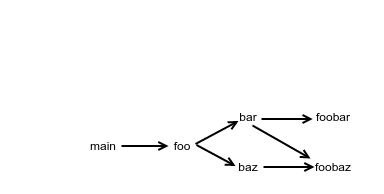
\includegraphics[width=3.5in, trim=0.8in 0in 0in 1.0in, clip]{callgraph.png}
\caption{The call graph of the example program}
\end{figure}

I define a potential error revealing method (PERM) as the method that might trigger the dynamic condition of residual investigation for a FindBugs bug pattern.  For example, FindBugs reports an error when a class overrides the equals(Object) method but not the hashCode() method.  Residual investigation installs dynamic checks for the condition that Object.hashCode() is called on an object of a class that redefines equals(Object) and inherits the implementation of hashCode(). The method that contains a call to hashCode() on the suspect class (i.e. the class that redefines equals and inherits hashCode) or its subclass is the PERM for this bug pattern.  Another example is that FindBugs statically detects dropped exceptions and reports them.  Residual investigation examines which methods end up being dynamically invoked in the suspect code block and watches whether the same methods ever throw the dropped exception when called from anywhere in the program. The methods that contain calls to a method that can be invoked in the suspect code block and can throw exceptions are the PERMs for this bug pattern. I analyze the PERMs using text search such as grep and static analysis such as call graph analysis and Java reflection API.  For example, for the dropped exception pattern, I analyze the types of the exceptions declared to be thrown by the methods in the suspect code block (suspect methods) using Java reflection and then search for methods whose names are the same as that of any suspect method and throw the same exceptions using grep.  Suppose the method foobar in the above code example is our PERM.  

Once finding a PERM, I interpose k levels back in the call graph from a PERM and call this a “switching” method.  Suppose k=1. In our example, the method bar is a switching method.  At the beginning I run existing system tests.  When I hit a switching method, I start exploring (i.e. switching to dynamic symbolic execution mode, instead of just dynamic execution).  To allow exploration, I relax (i.e., forget) some concrete values.  The first cut is to forget the arguments of switching methods.  In short, the invocation of a switching method turns on dynamic symbolic execution mode during the execution of an existing system test.  I declare victory when I find an approximate system test that calls the PERM method: the unit test case for bar that invokes foobar during its execution given the relaxed state.  In our example, this corresponds to a path like 

\begin{figure}[h]
\centering
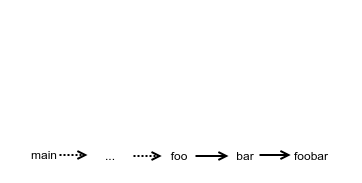
\includegraphics[width=3.5in, trim=0in 0in 0in 2.0in, clip]{path.png}
\caption{The path that calls the PERM method in the example program}
\end{figure}

The dotted line arrow marks the path before I start dynamic symbolic exploration (i.e. the path exercised by the existing system test), while the solid line arrow marks the path that the generated unit test case for bar establishes. 

PERM definitions for other bug patterns not mentioned in the above text:
\begin{itemize}
\item Bad Covariant Definition of Equals: FindBugs detects that programmers write equals method that accept a parameter of type other than Object.  Residual investigation checks whether the ancestral equals method, Object.equals(Object), is called on an instance of a class that has a covariant definition of equals.  The PERM for this bug pattern is the method that contains a call to equals() on the suspect class (i.e. the class redefines equals and inherits hashCode) or its subclass.
\item Cloneable Not Implemented Correctly: This bug pattern does not require native test suite.  Thus, I do not need to improve existing test suite.
\item Equals Method Overrides Equals in Super-class and May not Be Symmetric: FindBugs detects whether both the overriding equals method in the subclass and the overridden equals method in the superclass use instanceof in the determination of whether two objects are equal.  Residual investigation dynamically calls both equals method whenever it observes a comparison involving a contentious object and test if the results match.  The PERM for this bug pattern is the method that contains a call to equals() on the suspect superclass or subclass.
\item Non-Short-Circuit Boolean Operator: FindBugs issues warnings for use of \sv{\&} and \sv{|} inside the condition of an if statement.  Residual investigation checks for actual side-effects on the right-hand side of a non-short-circuiting boolean operator.  The PERM for this bug pattern is the method that contains a \sv{\&} or \sv{|} in an if statement.
\item Read Return Should be Checked: FindBugs checks if the return value from read in java.io.InputStream is ignored.  Residual investigation waits until it sees a read method on an object of any subclass of InputStream returns fewer bytes than requested (even for a call that does check the return value).  The PERM for this bug pattern is the method that contains a call to read on the suspect class.
\end{itemize}

\chapter{Related Work}
\label{chp:related}

Similar to us, hybrid concolic testing\cite{Majumdar:2007:HCT:1248820.1248874} interleaves random testing and concolic testing to increase coverage.  The switch from random testing to concolic testing happens when random testing does not find new coverage points after a predetermined steps; the switch from concolic testing to random testing happens when concolic testing finds an input to an uncovered branch goal (though concolic testing may need to explore several feasible execution paths to generate the new input).  But hybrid concolic testing is not designed to trigger one specific bug condition.  I are targeting at generating tests to trigger one specific bug condition, using call graph search and dynamic symbolic execution. 

\cite{Elbaum:2006:CDU:1181775.1181806} saves system test states and restores those states as regression tests.  I also save system test states.  But our purpose is helping setting up environment (i.e. assignments to heap variables) for starting dynamic symbolic execution of the “switching” method.

The closest work to us is \cite{Pasareanu:2008:CUS:1390630.1390635}, which uses system tests to set up the environment.  Different from\cite{Pasareanu:2008:CUS:1390630.1390635} that uses symbolic execution to generate unit tests, I use dynamic symbolic execution to generate unit tests.  This enables us to handle native method calls and some complicated constraints by replacing them with concrete values. 

\chapter{Management and Timeline}
\label{chp:timeline}

My overall goal is to defend the dissertation by September 2015.  I plan to submit a paper on the proposed work to ICSE 2016; the deadline for this conference is September 4, 2015.  Right now the underlying dynamic symbolic execution engine Dsc\cite{islam10dsc+mock} is similar to jCute\cite{sen06cute} released by University of Illinois at Urbana-Champaign. I plan to improve Dsc to make it become cutting-edge and open-sourced by the end of next March.  I plan to work out the required static analysis (e.g. call graph analysis) by May 2015.  I plan to finish the implementation of the proposed work by July 2015.  I will be writing the dissertation, performing implementations and evaluations, and plan to complete the dissertation by September 2015. 

\bibliographystyle{umthesis}
\bibliography{testing,testing-cc,refactoring,sigproc}

% History dates
%\received{February 2007}{March 2009}{June 2009}

% Electronic Appendix
%\elecappendix

\medskip

% that's all folks
\end{document}
